\documentclass[acmsmall,screen,review,anonymous,nonacm]{acmart}
\usepackage{amsmath,amsthm}
\usepackage{mathpartir}
\usepackage{listings}
\settopmatter{printacmref=false}
\renewcommand\footnotetextcopyrightpermission[1]{}


%% abbrevs
\newcommand{\system}{sys-name\xspace}

%% comments
% turn off comments by uncommenting the following command and
% commenting out the second notes command
%\newcommand{\notes}[2]{} 
% turn on comments by commenting out the previous note command and
% uncommenting the following command
\newcommand{\notes}[2]{{\bf\textsf{\textcolor{#1}{#2}}}} 
\newcommand{\todo}[1]{\notes{red}{TODO: #1}}
\newcommand{\milijana}[1]{\notes{teal}{Milijana says: #1}}
\newcommand{\sai}[1]{\notes{orange}{Sai says: #1}}
\newcommand{\reminder}[1]{\notes{purple}{Reminder: #1}}
\newcommand{\mathcomment}[1]{\notes{purple}{#1}}

%command to show the full definitions (first version) or not (second version)
%\newcommand{\extra}[1]{#1}
\newcommand{\extra}[1]{}

%% fonts
\newcommand\BbbGamma{\reflectbox{\rotatebox[origin=c]{180}{$\mathds L$}}}
\newcommand\BbbGammaVar{\reflectbox{\rotatebox[origin=c]{180}{$\mathbb L$}}}
\newcommand{\m}[1]{\mathsf{#1}}
\newcommand{\mt}[1]{\mathit{#1}}
\newcommand{\ft}[1]{\textit{#1}}
\newcommand{\paragraphb}[1]{\vspace{2pt}\noindent{\bf #1}\xspace}
%% math
\newcommand{\bnfdef}{::=}
\newcommand{\bnfalt}{\,|\,}
\newcommand{\rulename}[1]{\textsc{#1}}
\newcommand{\ifthen}[3]{\m{if}\ #1\ \m{then}\ #2\ \m{else}\ #3}
\newcommand{\while}[2]{\m{while}\ #1\ \m{do}\ #2}
\newcommand{\trans}[2]{\m{transition}(#1, #2)}
\newcommand{\elet}[3]{\m{let}\ #1 = #2 ~\m{in}\ #3}
\newcommand{\eletmut}[3]{\m{let~mut}\ #1 = #2 ~\m{in}\ #3}

%% typing 
\newcommand{\tctx}{\Gamma}
\newcommand{\pctx}{\Delta}
\newcommand{\Costarrow}[1]{\stackrel{#1}{\Rightarrow}}
\newcommand{\tctxdouble}{\BbbGamma}
\newcommand{\dgamma}{\BbbGamma}
\newcommand{\lbl}{\mathbb{L}}
\newcommand{\ilbl}[1]{\scriptsize\textit{#1}}
\newcommand{\lub}{\sqcup}
\newcommand{\entails}{\models}
\newcommand{\ok}{\m{ok}}
\newcommand{\subtp}{\sqsubseteq_t}


%% algo

%algo stuff 
% \usepackage{eqparbox}
% \newdimen{\algindent}
% \setlength\algindent{1.5em} 
% \algnewcommand\LeftComment[2]{%
% \hspace{#1\algindent}$\triangleright$ \eqparbox{COMMENT}{#2} \hfill %
% }

%% fonts
\newcommand{\alg}[1]{\ensuremath{\mathit{#1}}}


%% configurations
\newcommand{\prog}{\ft{prog}}
\newcommand{\seg}{\ft{seg}}
\newcommand{\dom}{\m{dom}}
\newcommand{\stepsto}{\longrightarrow}
\newcommand{\Stepsto}[1]{\stackrel{#1}{\Longrightarrow}}
\newcommand{\SeqStepsto}[1]{\stackrel{#1}{\longrightarrow}}
\newcommand{\MStepsto}[1]{\stackrel{#1}{\Longrightarrow^*}}
\newcommand{\MSeqStepsto}[1]{\stackrel{#1}{\longrightarrow^*}}
\newcommand{\proj}[2]{#1|_{#2}}
\newcommand{\stepstopc}[1]{\stackrel{#1}{\rightarrow}}

%% proofs
\newcommand{\ee}{\mathcal{E}}
\newcommand{\de}{\mathcal{D}}

\newcommand{\denote}[1]{[\![ #1 ]\!]}

\newcommand{\xstep}[1]{\xmapsto{#1}}
\newcommand{\xsteps}[1]{\xmapsto{#1}^*}
\newcommand{\step}{\mapsto}
\newcommand{\steps}{\mapsto^*}

\newcommand{\erase}[1]{{#1}^-}

\newcommand{\entry}[1]{\ft{Entry}(#1)}

\newcommand{\sametraceequiv}{\prec}
\newcommand{\twotraceequiv}{\approx}
\newcommand{\modeequiv}[1]{\approx_{#1}}
\newcommand{\outputequiv}{\approx^\m{out}}
\newcommand{\inputequiv}{\approx^\m{in}}



%% theorem environments

%%% proofs
\newif\ifproofs
%%%%%% uncomment to not show proofs 
%%\proofsfalse
%%%%%% uncomment to show proofs 
\proofstrue

\newtheorem{thm}{Theorem}
\newtheorem{lem}[thm]{Lemma}
\newtheorem{cor}[thm]{Corollary}

\newtheorem{defn}[thm]{Definition}
\newtheorem{assumption}[thm]{Assume}
\newenvironment{proofsketch}{\vspace{-1pt}\textsc{Proof (sketch). }\hspace*{0.25em}}{ \hspace*{\fill} \qed}

\newcommand{\myparagraph}[1]{\vspace{2pt}\noindent{\bf #1}}

\newcommand{\Cst}[2]{C(\text{#1} : \text{#2})}
\newcommand{\Ctr}[3]{C(\text{#1} : (\text{#2}, \text{#3}))}
\begin{document}

\title{Leveraging Types and Typestate for Peripheral Cost Analysis}
\author{Sai Divvela}
\email{sdivvela@terpmail.umd.edu}
\affiliation{\institution{University of Maryland} \city{College Park} \state{Maryland} \country{USA}}

\author{Milijana Surbatovich}
\email{milijana@umd.edu}
\affiliation{\institution{University of Maryland} \city{College Park} \state{Maryland} \country{USA}}
\setcctype{none}
\settopmatter{printacmref=false, printccs=false}
\maketitle

\input{sections/0_abstract}

\section{Introduction}
Automatic Resource Analysis has long been used to statically obtain bounds for the resource consumption of programs. Resources can mean a variety of relevant metrics, including the total energy used, the end-to-end execution time, or the maximum amount of memory consumed. Many techniques exist for obtaining these bounds, ranging from static analyses to program logics to type based approaches. \sai{cite sources} Type based approaches such as Automatic Amortized Resource Analysis (AARA) provide an appealing approach to deriving resource bounds, as they enable compositional reasoning while being able to support a large variety of programs. These approaches can be used to derive a wide variety of bounds, including upper, lower and tight bounds. The bounds that these approaches derive, and in particular upper bounds are useful in a number of contexts, including job scheduling, and resource sensitive contexts such as smart contracts or embedded systems. For embedded systems in particular, a robust understanding of the resource requirements are necessary, especially as battery-constrained IoT devices become increasingly popular and operate in resource-constrained environments. To operate effectively, these devices need a robust understanding of their energy requirements, commonly referred to as the Worst Case Energy Consumption (WCEC), which is the maximum possible charge across a given execution. A key challenge for determining the WCEC of a program however, is the usage of \textit{peripherals}, which are external devices such as sensors, radios, and actuators. Current works on determining the WCEC often utilize static analysis based approaches based on path enumeration. \sai{cite sources} While these approaches can offer strong guarantees, they often model peripherals in a very conservative manner, therefore limiting the tightness of their bounds. As mentioned previously, AARA provides an appealing approach due to it's compositional nature. However, it often lacks knowledge of peripherals, making it hard to apply directly to embedded systems.  

The key challenge here arises due to the stateful nature of many peripherals. This internal state determines not only how much power they draw from the main board, but also what operations they are able to perform. Prior work has partially addressed this problem through the lens of static analysis. WoCA \cite{woca} comes the closest, by integrating the stateful nature of peripherals directly into the analysis, allowing for the derivation of peripheral-aware energy bounds. Additionally, \cite{energy hoare logic paper} is also able to obtain device-aware energy bounds through the development of a program logic. In contrast to type-based systems though, these analyses are less able to be directly used out of the box, and place limitations on the expressiveness of programmers. 

Separately but related, there has been work on analyzing code for antipatterns to enable more energy efficient programming. Pudu \cite{pudu} is an analysis framework for the intermittent computing setting. In particular it aims to make reasoning about how peripherals use energy easier for developers by ensuring that all possible device states are tracked, so developers are never surprised by the behavior of the program. In the Pudu framework, there is a notion of a "burn bug" which refers to a peripheral using more energy than a programmer expected it to. 

To enable the reasoning of practical embedded systems programs without limiting developer expressivity, we introduce Heliod. Heliod to our knowledge is the first \textit{type system} to combine both typestate and cost analysis techniques in order to reason about programs that utilize peripherals. Heliod consists of the cost analysis type system, a core calculus to model important features in embedded systems programming including asynchronous peripheral operations and a changing device clock, and enables further optimizations of programs to eliminate burn bugs.

In order to reason about the stateful nature of peripherals, we utilize \textit{typestate}, a technique commonly used for encoding the runtime state of objects into it's type. By using typestate, programmers are able to specify how exactly each peripheral behaves, and the effect of the peripheral's internal state on the total cost of the program. Based on this definition, the type system is able to not just ensure that peripherals are used correctly with respect to their specification, but take advantage of this specification to provide a fine-grained cost accounting of the overall program. However, expecting programmers to have to constantly annotate the typestate whenever they write code would be burdensome, and could lead to costs being accounted for in a more conservative manner. As a result, we also developed a novel state inference algorithm which is able to infer what states each peripheral is in based on it's usage. This not only allows for easier programmability, but also allows us to derive tighter cost bounds as we solely look at how each peripheral is used. Using Heliod not only allows for the derivation of robust cost bounds based on the program behavior, but also allows for code to be checked for self-consistency w.r.t each peripheral's intended usage. 

To concretely summarize our contributions, they are: 
\begin{itemize}
  \item The first type system to utilize typestate and cost analysis in order to derive cost bounds for embedded systems
  \item A novel typestate inference algorithm that is able to accurately determine the states of peripheral devices, even when said state relies on non-local information
  \item A further analysis to find and warn about potential burn bugs, enabling programmers to optimize their code to be more efficient with respect to the cost model they choose
\end{itemize}


\section{Background}

We discuss how embedded systems and peripherals interact, and the challenge of providing peripheral-aware worst case energy consumption bounds, motivating the need to utilize typestate for a type-based approach to this problem. 

\subsection{Embedded Systems Basics}

An embedded system combines a processor with peripherals in order to perform actions such as timing, sensing and communication. The processor runs the main application code, and sends commands to peripherals to perform actions through the peripheral's API. However, not all commands are always valid for a given peripheral. For example, attempting to request a sensor to perform a measurement while it is turned off would fail. Many peripherals are \textit{stateful}, meaning they have an internal state that determines what commands can be accepted and performed. This internal state also determines the amount of power each peripheral draws from the main board as well. Importantly, this internal state can change either as a result of an API call, or by the hardware as a part of the peripheral's operation. This internal state is frequently represented as a state machine \sai{probably cite chibi here?}, and a simplified version of what such a state machine looks like for a common peripheral known as an I2C bus is shown in \autoref{fig:i2c_diagram}.
\begin{figure} \centering
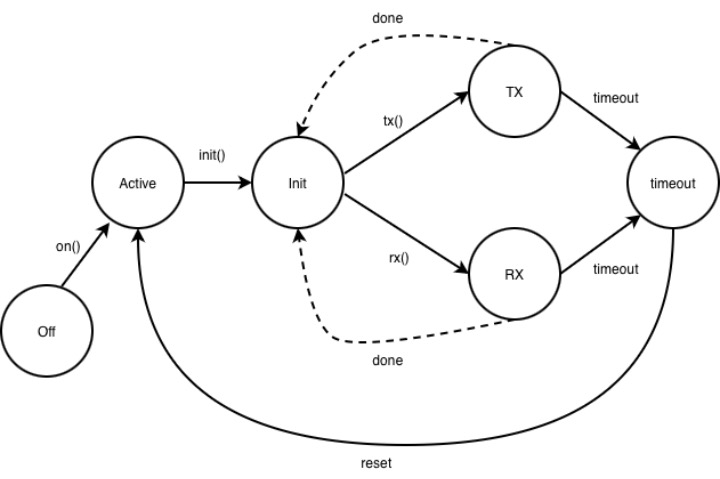
\includegraphics[width=0.5\linewidth]{diagram.jpeg} \caption{A simplified I2C bus state machine diagram}
\label{fig:i2c_diagram}
\end{figure}

Note that in the diagram, most edges are named with a specific function, this is because that function is what performs the state transition. However, the back-edges from the tx/rx state to the init state are represented with just "done." This is due to the hardware automatically transitioning back to the initalized state once it has finished performing it's action. Such transitions by hardware are common especially in low-power settings. In such settings, the processor will issue an initial command, and then continue to execute code until the hardware raises an interrupt that it has completed operation and transitioned back to a known state for the processor. When a peripheral is in a state where transitions are able to be performed by hardware, we call it \textit{unstable}, and we call states where transitions are only able to be performed by software \textit{stable}. Lastly, the processor clock affects the rate at which the processor executes cycles. This is important as certain peripherals such as the UART or I2C rely on the processor clock being a certain speed to operate correctly and efficiently. 

\subsection{Bounding Worst-Case Energy Consumption}

Worst-case energy consumption (WCEC) is the maximum energy a program can consume over its possible executions on a given platform. Broadly speaking, there are two main approaches to this problem. Measurement-based approaches estimate energy use by observing executions on hardware. The estimate depends on which inputs and device behaviors the measurements cover. Static analysis based approaches instead use a model of the program and hardware to bound the energy of possible executions. Recent work in this space has followed a similar high level structure: enumerate the possible runtime paths, and then translate into a formal constraint-satisfaction problem that can be solved when combined with hardware-specific information \cite{raffeck_et_al_OASIcs_WCET_2019_4,wegener_et_al_OASIcs_WCET_2023_9}.

For peripheral-aware analysis, the instructions executed by the processor only describe part of the system's activity. Peripherals consume energy when they perform work or change state, and they can continue to draw power while the processor executes unrelated code. The energy a peripheral consumes in a state depends on its power draw and how long it stays in that state. A clock change can affect the duration of processor work and, consequently, the time over which peripherals consume energy in the background. It can also affect the timing of peripherals that depend on the clock being changed. The primary approach that accounts for these factors is WoCA \cite{woca}, which uses peripheral state information combined with existing path enumeration techniques to provide a peripheral-aware energy consumption bound.

The actual bounds produced by prior work are largely derived from hardware-specific energy models, and provide concrete bounds in terms of the number of joules used. These can provide accurate bounds, but relies on such an energy model either being already present, or the user creating one for their own hardware. For Heliod, we instead opt to present costs in a symbolic manner. The major benefit of this symbolic cost calculation is that it enables relative reasoning of the energy consumption for the same program in a relatively hardware-agnostic manner. 

\subsection{Typestate and Type-Based Cost Analysis}

Typestate is a technique for encoding the runtime state of an object into the type system. This ensures that actions on a stateful object are only performed when the object is in the correct state. Abacus applies typestate to embedded peripherals by letting programmers describe device states and operations and generating Rust types that enforce those descriptions \cite{abacus}.

Type systems can also derive bounds on resource use. Automatic amortized resource analysis (AARA) associates potential with types and uses constraints generated during type inference to derive resource bounds \cite{Hoffmann_Jost_2022}. A cost semantics defines the resource consumed during execution and provides the basis for proving that a derived bound covers that cost.

Peripheral state gives a type-based energy analysis additional information about what to charge. Before a transition, the possible source states determine which transition costs the analysis must consider. While other code runs, the possible peripheral states determine which background costs it must include. This information also matters across function calls, since a function can receive a peripheral in different states at different call sites. Heliod uses typestate to carry this information into the analysis of both peripheral operations and their energy costs.

\section{Overview}

- Heliod Basics:
    - 3 main costs to consider
    - Simple example with synchronous code
    - Discuss how typestate and cost analysis go together
- State inference:
    - Motivate why we care with an example
    - Walk through how the example works
    - Talk about concretization
- Asynchronous Peripherals
    - We have hardware-software concurrency that we need to model
    - Discuss stable vs unstable states
    - Show with example on extending cost analysis and state inference to support this

\section{Language \& Type System Design} 

% Core calculus:
%     - Introduce syntax
%     - async/await for peripheral operations, explicit transition/downgrade statements
%     - Do not explicitly model rust ownership, but we assume it to be true
%     - Do not support unbounded loops/recursion due to their general lack of use in embedded programming
% Operational Semantics:
%     - Scheduler + stack of execution frames
%     - Model how embedded systems work to the best of our knowledge
%     - Explicit clock for timing, based on logical timesteps though
%     - Semantics are cost-aware, step charges a cost + advances the clock
% Typing:
%     - Important rules are transition/downgrade, function declaration, function call,  async, and await
%     - Explain how each of the rules work, state inference algorithm formally, and joining

Guided by our examples in Section 3, we present a core calculus to formalize this reasoning. We will first present the sequential fragment of our language, and then extend it to support asynchronous operations. 

\subsection{Sequential Heliod}
Our syntax for the sequential fragment is shown in ~\autoref{fig: syntax}. We include explicit \texttt{transition} and \texttt{downgrade} statements so that programmers can control when peripherals perform a state transition. To support dynamically inspecting peripheral state and performing actions based on it, we include a form of state ``pattern matching'' via $\texttt{match } p \texttt{ with } st_1 \mid \dots \mid st_n$. We assume that peripheral declarations are done all at once at the beginning of a program, and the names are globally scoped. Peripheral declarations also contain both a partial order $<$ and a set $D$ of downgrade policies. This is because we model the state machine of state transitions as a lattice with downgrading. Lastly, we also want to account for an embedded board's clock speed during the cost analysis. While this can get quite complicated, we support a simple abstraction through the \texttt{clock } $f$ command. This will set the clock speed to $f$---a non-zero rational number---and therefore allow for costs to be scaled by this new clock speed. 

\begin{figure}
\small
\[
\begin{array}{lcll}
\text{Peripheral Declarations: }p \bnfdef \ \text{id} \{\langle s_{0},s_{1},\ldots,s_{n}\rangle, <, st, D \}, p \ \vert \ \cdot 
\end{array}
\]
\[
\begin{array}{lcll}
\text{Declarations: }d & \bnfdef & \text{fn } f(e, p): \tau_1 \rightarrow \tau_2 \ \{c; ret := e\}, d \ \vert \ \cdot
\end{array}
\]
\[
\begin{array}{lcll}
\text{Commands: }c & \bnfdef & \text{let } x = e & \\ & \bnfalt & \text{let } x = f(e, p) \\ & \bnfalt & \text{if } e \text{ then } c_1 \text{ else } c_2  \\ & \bnfalt & \text{transition}(x, \text{st})  \\ & \bnfalt & \text{downgrade}(x, \text{st}) \\ & \bnfalt & \text{clock } f \\ & \bnfalt & \text{match }p \text{ with } \text{st}_1 \rightarrow c_1 | \dots | \text{ st}_n \rightarrow c_n  \\ & \bnfalt & c_1; c_2 
\end{array}
\]
\[
\begin{array}{lcll}
\text{Expressions: }e & \bnfdef & x \ \bnfalt \ v \ \bnfalt \ e_1 \text{ binop } e_2 
\end{array}
\]
\caption{Syntax}
\label{fig: syntax}
\end{figure}

To simplify our reasoning about peripheral devices, we assume a rust-like ownership model so aliasing is not a concern. The rules and language however do not explicitly model it. Our implementation targets real programs written in Rust, which must past the Rust typechecker, so any code that is analyzed will uphold this assumption. Importantly, the core language does not support unbounded loops, recursion, or higher-order functions. Unbounded loops are commonly used as a high level construct for managing scheduling, but Heliod is primarily meant for userspace applications where such loops are much less common, especially in safety critical applications. \cite{https://spinroot.com/gerard/pdf/P10.pdf} 

\paragraph{Typing Constructs}
We define the typing constructs for the sequential fragment of Heliod in \autoref{fig:constructs}. Peripheral devices have the type $\rho$ so we can determine when an operation is being performed on a peripheral. The constraints allow for state inference to be performed. Function types store not just the input and output base types, but also the input and output states---$\Vec{s_1}, \Vec{s_2}$---of the peripheral $p$ that is passed in. We store downgrade policies separately to align with our lattice model of transitions. Additionally, we assume the existence of cost functions $\m{cost}(s_i, s_j)$ which provides the cost of transitioning from state $s_i$ to state $s_j$ and $\m{cost}(s_i)$ which provides the cost of being in state $s_i$. 

\begin{figure}
\small
    \centering
\[
\begin{array}{llcl}
\textit{Typing Context} & \tctx & \bnfdef & x \rightarrow \tau, \tctx \bnfalt \cdot
\\ 
\textit{Types} & \tau & \bnfdef & \text{int} \bnfalt \text{bool} \bnfalt \text{unit} \bnfalt \rho \bnfalt (\tau_1, \Vec{s_1}) \rightarrow (\tau_2, \Vec{s_2})  
\\
\textit{Downgrade policy} & D & \bnfdef & s' \hookrightarrow s, D \bnfalt \cdot
\\
\textit{Peripheral Context} & \pctx & \bnfdef &  p \rightarrow \Vec{s}, \pctx \bnfalt \cdot
\end{array}
\]
\caption{Constructs}
\label{fig:constructs}
\end{figure}

\paragraph{Typing Rules} We present selected typing rules, primarily for function declarations and calls, transition/downgrade statements, and branching. In this version of Heliod, we have no state inference and no asynchronous operations yet. 
\begin{mathpar}
\inferrule*[left=T-Call]
{
\tctx(g) = (\tau_1, \Vec{s_1}) \rightarrow^{q_f(\cdot)} (\tau_2, \Vec{s_2}), f_f \\ \tctx,\pctx \vdash e : \tau_1, q_e \\ \pctx(p) = \Vec{s} \\ \Vec{s} \subseteq \Vec{s_1} \\ \pctx'_b = \pctx \setminus p \\ q = q_e + q_f[\pctx'_b]
}
{
\tctx,\pctx, f \vdash \text{let } x = g(e, p) : \text{unit} \Rightarrow \tctx[x : \tau_2], \pctx[p: s_2], q, f_f
}

\inferrule*[left=T-Transition]
{
\tctx,\pctx \vdash x : \rho \\ \pctx(x) = \Vec{s} \\ \text{stable}(st) \\ \forall s_i\in \Vec{s}, s_i \leq st \\ q = \max(\m{cost}(s_i, st))(f) + \m{cost}(\pctx \setminus x) + \m{cost}(\cdot)
}
{ 
\tctx,\pctx, f \vdash \text{transition}(x, st) : \text{unit} \Rightarrow \tctx, \pctx[x : st], q, f
}

\inferrule*[left=T-Downgrade]
{
\tctx,\pctx \vdash x : \rho \\ \pctx(x) = \Vec{s} \\ \forall s_i\in \Vec{s}, s_i \hookrightarrow st \in x(D) \\ q = \max(\m{cost}(s_i, st))(f) + \m{cost}(\pctx \setminus x) + \m{cost}(\cdot)
}
{ 
\tctx,\pctx, f \vdash \text{downgrade}(x, st) : \text{unit} \Rightarrow \tctx, \pctx[x : st], q, f
}

\inferrule*[left=T-If]
{
\tctx,\pctx \vdash e : \text{bool}, q_e \\ \tctx,\pctx \vdash c_1 : \tau \Rightarrow \tctx_1, \pctx_1, q_1, f_1 \\ \tctx,\pctx, f \vdash c_2 : \tau \Rightarrow \tctx_2, \pctx_2, q_2, f_2 \\ \tctx^* = \tctx_1 \cap \tctx_2 \\ \pctx^* = \pctx_1 \cup \pctx_2 \\ q = \max(q_1, q_2) + q_e + \m{cost}(\pctx) + \m{cost}(\cdot) \\ f^* = \max(f_1, f_2)
}
{
\tctx, \pctx \vdash \text{if } e \text{ then } c_1 \text{ else } c_2 : \tau \Rightarrow \tctx^*, \pctx^*, q, f^*
}

\inferrule*[left=T-FunDecl]
{
\tctx[x : \tau_1], \pctx[p: \Vec{s_1}], \beta: \text{amb}, f \vdash c: \tau_2 \Rightarrow \tctx', \pctx', f_f, q_1(\cdot) \\ \pctx'(p) = \Vec{s_2} \\ \tctx', \pctx' \vdash e : \tau_2, q_2(\cdot) \\ q_f = (q_1 + q_2)(\cdot)
}
{ \tctx,\pctx, f \vdash \text{fn } f(x, p) : (\tau_1, \Vec{s_1}) \rightarrow (\tau_2, \Vec{s_2}) \  \{c; ret := e\} \Rightarrow \tctx[f \mapsto (\tau_1, \Vec{s_1}) \rightarrow^{q_f} (\tau_2, \Vec{s_2}), f_f], \pctx
}
\end{mathpar}

\section{Correctness}
\subsection{Operational Semantics and Assumptions}
\subsection{Type Safety}
\subsection{Cost Soundness}
\subsection{Cost Accounting and Bound Precision}


\begin{thm}[Type Soundness]
\label{thm:type-soundness}
Suppose $c$ checks under valid function signatures and
\[
\tctx, \pctx, f \vdash c
\Rightarrow \tctx', \pctx', q_c(f,\beta), f_c(f).
\]
If the initial store and peripheral state agree with $\tctx$ and
$\pctx$, then $c$ has a terminating evaluation. Every evaluation from
these initial conditions ends in a store and peripheral state that
agree with $\tctx'$ and $\pctx'$. Its actual cost $q$ and exit clock
$f'$ satisfy
\[
q \leq q_c(f,\beta)
\qquad
f' \leq f_c(f).
\]
\end{thm}

\begin{thm}[Inference Soundness]
\label{thm:inference-soundness}
Suppose state inference derives output contexts $\tctx', \pctx'$
and summaries $q_c, f_c$ for $c$ under input contexts $\tctx, \pctx$.
If $c$ evaluates at clock $f$ with ambient background cost $\beta$
from a store and peripheral state that agree with $\tctx$ and $\pctx$,
then the final store and peripheral state agree with $\tctx'$ and
$\pctx'$. Its actual cost $q$ and exit clock $f'$ satisfy
\[
q \leq q_c(f,\beta)
\qquad
f' \leq f_c(f).
\]
\end{thm}

\begin{thm}[Slack Decomposition]
\label{thm:slack-decomposition}
Suppose a sequential program checks with cost summary $q_{\m{main}}$
and evaluates from its initial configuration at clock $f_0$ with
actual cost $q$. There is a finite list $L$ of slack items for the
execution. Each item $i \in L$ records a typed charge
$q_i^{\m{typed}}$ and an actual charge $q_i^{\m{actual}}$, with
$q_i^{\m{actual}} \leq q_i^{\m{typed}}$. Since the program starts with
zero ambient background cost,
\[
q_{\m{main}}(f_0,0)
=
q + \sum_{i \in L}
\bigl(q_i^{\m{typed}} - q_i^{\m{actual}}\bigr).
\]
\end{thm}

\section{Implementation}
We implemented Heliod as a compile-time analysis inside of Abacus \cite{abacus}, a framework for typestate-based peripheral programming that uses Rust's procedural macro system. Heliod operates on a function's raw syntax tree, applying state inference and cost analysis rules to each visited node. Once completed, the code is passed through to the Rust type checker so that the code remains consisten with Rust's ownership and borrowing semantics. We primarily used Heliod on peripherals that are supported by Embassy, which is a Rust framework for developing embedded systems applications.

\subsection{Using Heliod}

To use Heliod, a programmer annotates a function, implementation block, or inline module with \texttt{\#[heliod(PeripheralCost)]}. Peripherals are declared using Abacus’s \texttt{process\_register\_block} machinery, which already provides state and substate declarations, stable and transient classifications, and register-operation permissions. Heliod reuses these as they are. The transition and downgrade lattice of Section 3 is shorthand for the same finite-state machine, so Heliod keeps no separate downgrade policy specification. Heliod adds a background cost to each state and a foreground cost to each operation. Costs may be a number of ticks or symbolic variables. Depending on how costs are provided, bounds are reported accordingly.  Furthermore, the programmer does not annotate peripheral states at use sites. A peripheral parameter without explicit annotations uses state inference to determine the set of states that the peripheral is in.

\subsection{Limitations \& Differences from the Formal Model}
The implementation and core calculus are closely related, however differ in a couple of important ways. First, due to how Embassy autogenerates register APIs using a PAC crate, Heliod is unable to be applied directly to the individual register accesses. The Abacus framework expects a fully annotated MMIO type to store all of the relevant information. While we could have reimplemented Embassy's autogenerated API to an annotated MMIO type, that would be difficult and potentially error-prone. Instead, Heliod is applied to internal helpers, which are small collections of register accesses and operations that compose together to form a well-defined API for the peripheral under analysis. These helpers declare their effect with \texttt{\#[heliod\_operation(peripheral, from, to, cost, background\_steps)]}, where \texttt{from} and \texttt{to} are states and \texttt{cost} can be either a symbolic cost variable or a number of ticks. the \texttt{background\_steps} is required as operations can last for more than one step, and specifying the number allows the analysis to propagate the background charge accurately. These are trusted contracts that Heliod uses to build up the cost analysis. 

For the actual analysis, the implementation is also able to reason about bounded loops by essentially performing loop unrolling. For unbounded loops, the implementation is able to reason about such loops where peripherals return to the same state they started in at the beginning of the loop, and there are no early returns. In such cases, Heliod will return a per-iteration bound to help aide developers. The implementation and model do not support more complex features of Rust, including arbitrary unsafe code, generics, closures, recursion and general trait implementations. However, Heliod allows for the use of the \texttt{heliod\_operation} macro as a contract for opaque functions which lie outside of Heliod's analysis, therefore allowing it to integrate with code it hasn't checked. 

\paragraph{Async Support}
Because Heliod needs to reason about hardware-software concurrency, it has a limited form of support for the Rust async/await programming model. Heliod is able to reason about asynchronous functions that are immediately awaited, along with Embassy's \texttt{OnDrop} and \texttt{with\_timeout()} fallback constructs for asynchronous programming. However anything beyond that is currently unsupported.

\section{Evaluation \& Case Studies}

We perform case studies on the NRF 52840dk board. 

- implement heliod for both UART and temperature sensor \\
- temperature sensor produces costs purely symbolically, UART uses a tick-based model, show that we can get cost derivations for each peripheral API \\
- combining these into an actual application, show that we get application level bounds \\
- discuss and show burn bug analysis, current burn bugs are just planted. hopefully show how the optimizations leads to directionally less energy consumed \\
- show the relative overhead of heliod compared to not using it. hopefully this is small to negative

\section{Related}

\section{Conclusion}

\end{document}